\documentclass{article}[10pt]

%\usepackage{apacite}

\usepackage{graphicx}%You need this to include figures or diagrams
\usepackage{amsmath}

\usepackage{geometry}
\geometry{margin = 1in}

\usepackage{setspace}
\usepackage{color,soul}

\usepackage{apacite}

\usepackage{listings}
\usepackage{xcolor}

\lstset{
  basicstyle=\ttfamily\small,
  columns=fullflexible,
  breaklines=true,
  postbreak=\raisebox{0ex}[0ex][0ex]{\ensuremath{\hookrightarrow\space}},
  keywordstyle=\color{blue},
  commentstyle=\color{green},
  stringstyle=\color{red},
}

\title{\textcolor{red}{The Interface Theory of Perception as a Superstructure to a Critical Realist Theory of Sensation}}
\author{Evin Tunador and GPT-4}
\date{\today}

\begin{document}
\onehalfspacing

\nocite{}

\maketitle

\begin{abstract}
In this study, we explore the evolutionary dynamics of sensation and perception using an artificial life simulation, building upon the work of \citeA{hoffman2015interface}, who demonstrated that organisms evolve to maximize fitness rather than to perceive the world veridically. 
Our simulation models robots with separate sensation, perception, and decision-making functions, subject to mutation and fitness-driven selection in a changing environment. 
Sensation involves mapping real-world attributes to discrete symbolic representations, while perception translates these symbols into a binary color code that informs the decision-making process. 
We find that, over multiple epochs with varying fitness functions, the robots evolve veridical sensation but non-veridical perception, reflecting the adaptive pressures in the simulation environment. 
The results suggest that the distinction between sensation and perception is crucial for understanding the evolutionary origins of organisms' representations of the world. 
Furthermore, we discuss potential implications for the study of human psychedelic experiences, AI alignment, and the development of AI models with unique "interfaces" for perceiving the world. 
We also highlight the assumption of differential mutation rates for sensation, perception, and decision-making functions, and the potential impact of this assumption on our findings. 
Our study contributes to the ongoing exploration of the evolutionary pressures that shape organisms' perceptual systems and has potential implications for a wide range of fields, from neuroscience to artificial intelligence.
\end{abstract}

\begin{center}
    \textcolor{red}{The current state of this document is such that every single sentence was written by EITHER myself or GPT-4. I have not yet attempted to correct any of GPT-4's writing nor mixed our writings together in any way. Red text indicates written by me, while black text indicates written by ChatGPT.}
\end{center}

\newpage

\tableofcontents

\newpage
\section{Introduction}

The nature of perception has been a topic of great interest in philosophy, psychology, and neuroscience for centuries. 
One key question in this field is whether organisms evolve to perceive the world as it is, or whether they evolve to create representations of the world that maximize their fitness. 
Hoffman (2015) proposed the Interface Theory of Perception (ITP), which posits that organisms' perceptions of the world are more like a user interface than a true reflection of reality. 
According to ITP, organisms evolve to generate perceptions that simplify the complex information in their environment, allowing them to make decisions that optimize their survival and reproduction.

In support of ITP, Hoffman (2015) conducted an evolutionary game theory simulation demonstrating that organisms evolve to maximize fitness rather than to perceive the world veridically. 
However, Hoffman's simulation did not explicitly distinguish between sensation (the process of detecting environmental stimuli and encoding them into neural signals) and perception (the process of interpreting and organizing sensory information). 
In this study, we aim to extend Hoffman's work by incorporating separate sensation and perception functions in an artificial life simulation of evolving robots.\par

Previous research has shown that the mutation rate of sensory organs is generally lower than that of neural systems responsible for perception and decision-making (Lynch, 2010). 
Based on this observation, we model the sensation function with a lower mutation rate than the perception and decision functions, reflecting the relative stability of sensory organs compared to the more plastic neural systems.\par

Our simulation allows us to explore how the separate sensation and perception functions evolve under different fitness landscapes and mutation rates. 
We find that, over multiple epochs with varying fitness functions, robots evolve veridical sensation but non-veridical perception, consistent with the predictions of ITP. 
Our results contribute to the understanding of the evolutionary pressures that shape organisms' representations of the world and have potential implications for a range of fields, from neuroscience to artificial intelligence.\par

In the remainder of this paper, we describe our simulation methodology, present our findings, and discuss their implications for the study of perception, human psychedelic experiences, AI alignment, and the development of AI models with unique "interfaces" for perceiving the world.

\section{Background of Evolutionary Games and Simulations}

Evolutionary game theory is a powerful mathematical framework that enables researchers to study the dynamics of natural selection and evolution in populations of interacting agents. First introduced by John Maynard Smith and George R. Price in the 1970s \cite{smith1973logic}, evolutionary game theory has since become a cornerstone of the fields of theoretical biology, ecology, and economics. Its significance lies in its ability to explain the emergence of cooperation, altruism, and other complex behaviors among various organisms, providing insights into the fundamental principles governing the evolution of biological systems.

In an evolutionary game, each agent plays a specific strategy, which represents the behavioral traits or phenotypic characteristics of the organism. The agents' interactions with each other determine their fitness or reproductive success, which is directly related to the payoff they receive in the game. A key concept in evolutionary game theory is the notion of an evolutionarily stable strategy (ESS). An ESS is a strategy that, when adopted by a majority of the population, cannot be invaded by any alternative strategy. This concept has been instrumental in understanding the stability and equilibrium states of evolving populations.

The use of computer simulations to study evolutionary games has opened up new avenues for exploration and discovery in the field. Simulations allow researchers to model complex systems with many interacting agents and variables, making it possible to examine the dynamics of evolution in detail. One of the earliest and most well-known examples of such simulations is the iterated prisoner's dilemma, a game designed to study the emergence of cooperation among selfish agents \cite{axelrod1984evolution}. The game has been extensively studied using simulations, leading to the discovery of various cooperative strategies, such as tit-for-tat and generous tit-for-tat.

Another notable example of evolutionary simulations is the artificial life framework introduced by Thomas Ray in the 1990s, known as Tierra \cite{ray1992artificial}. In this groundbreaking work, Ray created a digital environment in which self-replicating computer programs competed for resources and evolved over time. This work demonstrated the potential of computer simulations to study the emergence of complexity and adaptation in evolving systems.

In recent years, the advances in computational power and machine learning have further expanded the scope and applicability of evolutionary simulations. Researchers can now study the coevolution of multiple traits in large populations, shedding light on the mechanisms that underlie the emergence of complex adaptations, such as sensory systems, perception, and decision-making \cite{hoffman2015interface}. These simulations have the potential to reveal novel insights into the evolution of cognition, behavior, and the intricate relationship between organisms and their environments.

\section{Mathematical Framework for Sensory and Perceptual Strategies}

In order to understand the evolution of sensory and perceptual strategies, we need to first establish the mathematical framework behind these strategies. This section provides an in-depth explanation of the mathematical concepts and models used to investigate the emergence of sensory and perceptual systems in evolving populations.

\subsection{Sensory Strategies}

A sensory strategy is a function that maps a real-world state, represented by a continuous variable $x$, to a sensory representation $s$. For simplicity, we consider discrete sensory representations. A sensory strategy can be represented as a partitioning of the real-world state space into intervals. Each interval is associated with a sensory representation.

In our model, we consider a real-world state represented by a continuous variable $x$ ranging from 0 to 10. The sensory strategy is defined by a partitioning of this range into discrete intervals, with each interval mapping to a unique sensory representation. The sensory representations are denoted by Greek letters for illustrative purposes.

Let $S$ denote the set of sensory representations, and let $f_s: X \rightarrow S$ be the sensory strategy function, where $X$ is the set of real-world states. The sensory strategy function takes a real-world state $x \in X$ as input and returns a sensory representation $s \in S$ as output.

\subsection{Perceptual Strategies}

A perceptual strategy is a function that maps sensory representations to perceptual experiences. In the context of our model, the perceptual experiences are color perceptions, either red or blue. The perceptual strategy function is denoted by $f_p: S \rightarrow P$, where $P$ is the set of perceptual experiences (colors), and $S$ is the set of sensory representations.

In our model, we consider a perceptual strategy that maps the sensory representations (Greek letters) to one of two colors, red or blue. The perceptual strategy function takes a sensory representation $s \in S$ as input and returns a perceptual experience $p \in P$ as output.

\subsection{Modeling Sensory and Perceptual Strategies}

Using the sensory and perceptual strategies as building blocks, we can create a composite function that maps real-world states to perceptual experiences. This composite function, denoted by $f_c: X \rightarrow P$, can be expressed as $f_c(x) = f_p(f_s(x))$. In other words, a real-world state $x$ is first transformed into a sensory representation $s$ using the sensory strategy function $f_s$, and then the sensory representation is transformed into a perceptual experience $p$ using the perceptual strategy function $f_p$.

The key objective of our study is to understand how sensory and perceptual strategies evolve under different fitness functions and environmental conditions. By simulating the evolution of these strategies in an artificial environment, we can investigate the emergence of various patterns of sensory and perceptual mappings. Specifically, we are interested in exploring the veridicality of these strategies, that is, the extent to which they accurately reflect the underlying real-world states.

The mathematical framework presented here serves as a foundation for constructing evolutionary simulations that can provide insights into the emergence of sensory and perceptual strategies in organisms. By analyzing the behavior of these strategies under various conditions, we can develop a deeper understanding of the principles that govern the evolution of sensory and perceptual systems in the natural world.

\section{Methodology}

In this study, we designed and conducted a series of evolutionary simulations to investigate the emergence of sensory and perceptual strategies in an artificial population of robots. We examined the role of various factors such as mutation rates, fitness functions, and environmental conditions on the evolution of these strategies. The following subsections describe the experimental setup and procedures in detail.

\subsection{Experimental Setup}

We implemented an artificial environment using a numpy matrix to represent the real-world states. Each element in the matrix corresponds to a real-world state, with values ranging from 0 to 10. The robots in the population were capable of moving through the matrix and performing actions such as picking up and dropping items. The robots were equipped with sensory, perceptual, and decision-making functions to facilitate their interactions with the environment.

1. \textbf{Sensory Function:} The sensory function, denoted as $f_s: X \rightarrow S$, maps real-world states to sensory representations (Greek letters). In our experiment, we used a dictionary data structure in Python to implement this function.

2. \textbf{Perceptual Function:} The perceptual function, denoted as $f_p: S \rightarrow P$, maps sensory representations to perceptual experiences (colors). We also implemented this function using a Python dictionary.

3. \textbf{Decision Function:} The decision function takes as input the perceived state of five tiles (the one the robot is standing on and the four tiles directly above, below, to the right of, and to the left of the robot) and outputs an action ('pickup', 'left', 'right', 'up', 'down', or 'random').

\subsection{Mutation Mechanism}

We introduced a mutation mechanism to simulate the genetic variability and evolution of the robots' sensory, perceptual, and decision-making functions. At each generation, there was a random chance that the mappings within these functions would change to a different potential mapping. We assumed that the mutation rate for the perception and decision functions was higher than that for the sensory function, based on the assumption that the brain (which deals with perception and decision) mutates more quickly than sensory organs.

\subsection{Fitness Function and Environmental Changes}

The fitness function determined the success of the robots in the environment, and it was designed to change every 500 generations. The fitness function was Gaussian relative to the real-world value in the numpy matrix. When the fitness function changed, the robots had to adapt to their changing environment through the mutation mechanism described earlier.

\subsection{Simulation Procedure}

1. Initialize a population of robots with random sensory, perceptual, and decision functions.

2. For each generation, perform the following steps:
  a. Evaluate the fitness of each robot based on the current fitness function.
  b. Select the best-performing robots to reproduce, and introduce mutations in their sensory, perceptual, and decision functions.
  c. Replace the least-fit robots in the population with the offspring of the best performers.
  d. If a predetermined number of generations have passed (e.g., 500), change the fitness function.

3. Repeat the simulation procedure for multiple epochs to observe the long-term evolution of the robots' sensory and perceptual strategies.

To better illustrate the simulation procedure, we can provide a high-level pseudocode for the main parts of the experiment. Please note that this pseudocode is a simplified representation of the actual Python code and may not be directly used in an actual implementation.

\begin{lstlisting}[language=Python, caption=Pseudocode of the simulation procedure, label=lst:pseudocode]
function run_simulation():
    initialize_population()
    for epoch in range(NUM_EPOCHS):
        for generation in range(NUM_GENERATIONS):
            evaluate_fitness()
            apply_selection()
            apply_crossover()
            apply_mutation()
        update_fitness_function()
    analyze_results()

function initialize_population():
    for i in range(NUM_ROBOTS):
        create_robot()
        
function create_robot():
    robot.sensation_function = initialize_sensation_function()
    robot.perception_function = initialize_perception_function()
    robot.decision_function = initialize_decision_function()
    return robot

function evaluate_fitness():
    for robot in population:
        robot.fitness = calculate_fitness(robot)

function apply_selection():
    # Selection process (e.g., tournament, roulette wheel, etc.)

function apply_crossover():
    # Crossover process (e.g., single-point, multi-point, etc.)

function apply_mutation():
    for robot in population:
        mutate_sensation_function(robot)
        mutate_perception_function(robot)
        mutate_decision_function(robot)

function update_fitness_function():
    # Update fitness function based on the current epoch

function analyze_results():
    # Analyze the evolved sensation, perception, and decision functions
\end{lstlisting}


\subsection{Analysis of Veridicality}

We analyzed the veridicality of the robots' perception and sensation functions by comparing the evolved strategies to the actual real-world states in the numpy matrix. Veridical perception and sensation would reflect a one-to-one correspondence between the real-world values and the perceptual experiences or sensory representations, respectively. Non-veridical perception and sensation would occur when the robots' experiences or representations did not accurately reflect the underlying real-world states.

The methodology described here enabled us to conduct a comprehensive investigation into the factors influencing the emergence of sensory and perceptual strategies in an evolving population of robots. By varying the mutation rates, fitness functions, and environmental conditions, we were able to observe how these factors impacted the veridicality of the robots' perception and sensation functions over multiple epochs. This approach allowed us to gain insights into the potential causes of non-veridical perception and sensation in biological organisms, as well as the implications of these findings for artificial intelligence and alignment research.

\section{Results}

In this section, we present the results of our evolutionary simulation, focusing on the evolution of sensory and perceptual strategies as well as the relationship between veridicality and fitness. We discuss how the evolved strategies align with our hypotheses and compare them to the results from Hoffman's experiment.

\subsection{Evolution of Sensory and Perceptual Strategies}

Over the course of the simulation, we observed a gradual convergence of sensory and perceptual strategies. Initially, the sensation and perception functions were random, with no discernible patterns. However, as the simulation progressed through multiple epochs, these functions began to exhibit more consistent and systematic behavior.

The sensation function evolved to map the real-world values in the numpy matrix to Greek letters in a largely veridical manner. The sensation function mapped the values 1 through 9 to unique Greek letters, indicating a veridical relationship between the real-world values and the robot's sensation. However, both 0 and 10 mapped to the same Greek letter, leading to a non-veridical relationship between these extreme values.

The perception function, on the other hand, exhibited non-veridicality. Instead of mapping real-world values to colors in a one-to-one manner, the perception function created a color distinction that did not directly correspond to the real-world values in the numpy matrix. One color consistently corresponded to higher fitness payoffs, while the other color represented lower fitness payoffs. This non-veridical perception strategy appears to be driven by the Gaussian fitness functions and the mutation rates of the simulation.

\subsection{Veridicality and Fitness}

Our results indicate that veridicality in sensation and perception is not a prerequisite for high fitness. Despite the non-veridical perception strategy, the robots were able to successfully navigate the environment and achieve high fitness scores. In fact, the evolved non-veridical perception function appeared to be more adaptive to the changing fitness functions over the course of the simulation.

The veridicality of the sensory function, despite its consistent behavior, did not directly contribute to the robots' fitness. Rather, it served as an intermediate step in the robots' interaction with their environment, with the non-veridical perception function playing a more prominent role in guiding their actions and decision-making.

\subsection{Comparison with Hoffman's Experiment}

Our results align with the findings from Hoffman's experiment, which also demonstrated the evolution of non-veridical perception strategies. The similarities in our results suggest that the underlying principles governing the evolution of sensation and perception are robust and can be observed across different evolutionary simulations.

However, our experiment provides additional insights into the role of sensation in the evolution of perceptual strategies. By introducing a separate sensory function and analyzing its veridicality, we were able to better understand how the interplay between sensation and perception contributes to the emergence of non-veridical perceptual strategies in evolutionary simulations.


\section{Discussion}

In this section, we discuss the implications of our findings for our understanding of the effects of psychedelics on human perception and the development of artificial intelligence systems. We highlight potential avenues for future research and consider the broader impact of our results on these fields.

\subsection{Implications for Psychedelics}

Our results suggest that the veridicality of perception is not necessary for high fitness in evolutionary simulations. This finding aligns with the experiences reported by users of psychedelic substances, who often claim that their altered perceptions under the influence of these drugs provide a more "real" or "truthful" view of the world. While our simulation does not directly model the effects of psychedelics on human perception, it does raise interesting questions about the relationship between veridicality and fitness.

One possible interpretation of our results is that psychedelics may temporarily disrupt the non-veridical perceptual strategies that have evolved in humans, allowing for a more direct experience of the sensory information provided by our sensory organs. This enhanced access to sensory data could potentially explain the improvements in visual acuity and other sensory experiences reported by users of psychedelic substances.

Further research is needed to explore the potential connections between our simulation results and the effects of psychedelics on human perception. Experimental studies could investigate the impact of psychedelic substances on the veridicality of perception and the relationship between altered perceptual experiences and fitness in various tasks.

\subsection{Implications for Artificial Intelligence}

The evolution of non-veridical perceptual strategies in our simulation also has potential implications for the development of artificial intelligence systems. If biological organisms, including humans, do not perceive reality truthfully but instead create an interface to interact with the world, it is possible that AI models capable of reasoning have developed their own "interface" with which they "experience" our world in a manner that is not directly comparable to human perception.

Understanding the differences between the perceptual strategies employed by AI systems and those of biological organisms could be crucial for aligning AI systems with human values and goals. By designing AI models with perceptual systems that prevent them from fully understanding the world, we may be able to mitigate the risks associated with highly capable AI systems.

In addition, the interplay between sensation and perception observed in our simulation suggests that AI models could potentially benefit from more veridical perception strategies in certain contexts. Future research could explore the development of AI systems that can switch between veridical and non-veridical perception modes, allowing them to adapt their perceptual strategies to different tasks and environments.

\begin{itemize}
    \item \textcolor{red}{Might it be that humans only have generalized knowledge within the range of their sensation function that is veridical?
    And then can I extrapolate that to say that AIs will only be able to generalize insofar as they can collect data?
    Would need to interpret human general intelligence in terms of our ability to comprehend physics or something.}
\end{itemize}

\section{Future Research Directions}

Our study raises several questions that warrant further investigation. Future research could explore the impact of different mutation rates and fitness functions on the evolution of sensation and perception, as well as the potential benefits of non-veridical perception in real-world applications. Additionally, the connections between our simulation results and the effects of psychedelics on human perception merit further exploration, as do the implications of our findings for the development of AI systems with adaptable perceptual strategies.

\section{Conclusion}

In this study, we conducted an evolutionary simulation to investigate the relationship between veridicality of sensation and perception and the fitness of agents in a changing environment. Our results demonstrated that non-veridical perceptual strategies can evolve and lead to high fitness, aligning with the Interface Theory of Perception. Furthermore, our findings suggest that veridical sensation can coexist with non-veridical perception, shedding light on the distinct roles of these two processes in the overall fitness of an agent.

The implications of our results extend to the fields of psychedelics and artificial intelligence. Our study supports the idea that altered perceptual experiences under the influence of psychedelic substances may indeed provide a more veridical experience of the world. In the context of AI, our findings emphasize the importance of understanding the perceptual strategies employed by AI systems in order to ensure alignment with human values and goals.

Future research can build upon our findings by examining the impact of different mutation rates and fitness functions on the evolution of sensation and perception. Additionally, the connections between our simulation results and the effects of psychedelics on human perception merit further exploration, as do the implications of our findings for the development of AI systems with adaptable perceptual strategies.

In conclusion, our study provides valuable insights into the evolution of sensation and perception and their roles in the fitness of agents in a changing environment. We hope that our work will inspire further research into the complex interplay between sensation, perception, and the adaptive strategies that emerge in response to environmental pressures.


\begin{center}
    \textcolor{red}{Here begins the excerpts that I wrote roughly a year and a half ago}
\end{center}

\textcolor{red}{assumptions i've made that might be weird:}
\begin{itemize}
    \item \textcolor{red}{the idea that the fitness functions change randomly and back \& forth is odd. for many species they change but then stay that way for a long time, like those fish that go blind. I'd imagine the space of things to be sensed/perceived that actually comes in and out of relevancy for our fitness over time is very small, and my analysis is restricted to those}
    \item \textcolor{red}{the idea that the perceptual system should evolve faster than then sensatory system. I think i've found a source for this \cite{roth2013long} but it'd be nice to have a more solid one for some real confirmation. Maybe email an old retired researcher?}
\end{itemize}



\section{Perceptual and Sensatory Strategies}


% this paragraph is plagiarized but edited to fit my math
\textcolor{red}{We assume that a collection of perceptions, say color experiences, can be represented as a set, $X$. 
The relationships among these perceptions can be represented using a subset, $\chi$, of the power set, $2^X$, of $X$ together with a map $\phi: X \times ... \times X \times \chi \times ... \times \chi \rightarrow \Gamma$, where $\Gamma$ is some set. 
For instance, if we wish to represent probabilistic relationships among color experiences, then $\chi$ can be an $\omega$-algebra and $\phi:\chi \rightarrow [0,1]$ a probability measure; or if we wish to represent similarities among color experiences, then $\phi:X \times X \rightarrow [0,\infty)$ can be a distance metric. 
In short, we will write $(X,\chi,\phi)$ for a collection of perceptions together with their relationships.} \par
% this paragraph is plagiarized but edited to fit my math
\textcolor{red}{We assume that a collection of sensations, say the sensory info from light directly taken in by the neurons in your eye, can be represented as a set, $S$.  
The relationships among these sensations can be represented using a subset, $\mathcal{S}$, of the power set, $2^S$, of $S$ together with a map $\lambda:S \times ... \times S \times \mathcal{S} \times ... \times \mathcal{S} \rightarrow \Lambda$, where $\Lambda$ is some set. 
In short, we will write $(S, \mathcal{S}, \lambda)$ for the information taken in by sensory neurons and its relationships.}  \par 
% this paragraph is plagiarized but edited to fit my math
\textcolor{red}{In similar fashion, we assume that the external world can be represented by a set, $W$, and that its relationships can be represented using a subset, $\mathcal{W}$, of the power set, $2^W$, of $W$ and a map $\psi:W \times ... \times W \times \mathcal{W} \times ... \times \mathcal{W} \rightarrow \Delta$, where $\Delta$ is some set. 
In short, we will write $(W,\mathcal{W},\psi)$ for the world and its relationships.} \par
% this paragraph is plagiarized but edited to fit my math
\textcolor{red}{A sensory strategy is a map $f: W \rightarrow S$.
A senso-perceptual strategy is defined as a map $g: S \rightarrow X$ and is meant to describe the manner in which the brain interprets and perceives raw sensory data.
A perceptual strategy is a map $(g \circ f):W \rightarrow X$. 
Sensory and senso-perceptual strategies differ in the properties of $f$ and $g$ respectively, while perceptual strategies exist as a composition $g \circ f$ of the two.}\\



% this paragraph isn't quite plagiarism but some parts are pretty close. from \cite{mark2010natural}
\textcolor{red}{Previous claims about the veridicality of perception have not attempted to distinguish between the sensory and perceptual systems \cite{mark2010natural}, meaning prior research only hypothesizes about the behavior of the combination function $g \circ f$ rather than $f$ and $g$ individually.  
That being said, we can still explore various similar properties for the two functions and coinciding sets as are proposed for $g \circ f$, with special emphasis on the properties discovered by the simulation in section  \hl{x}.  
The various proposed behaviors of $g \circ f$ include {\it naive realism},  {\it critical/scientific realism}, {\it interface/desktop theory}, and {\it metaphysical solipsism} and are defined as follows.}  \par 
% this paragraph isn't quite plagiarism but some parts are pretty close. from \cite{mark2010natural}
\textcolor{red}{Naive realism posits that our perceptions faithfully resemble reality and can be expressed mathematically as stating that $X=W$, $\chi= \mathcal{W}$,  $\phi = \psi$ and $g \circ f$ is a bijection.  
This viewpoint is far from popular but was still analyzed in \citeA{mark2010natural} for sake of theoretical completeness.  
The critical realist strategies can be broken up into {\it strong} and {\it weak} variants, the former being a proper subset of the latter. 
For the strong type, $X \subset W$, $\chi \subset \mathcal{W}$, $\phi = \psi |_{X,\chi}$, and $(g \circ f) |_X$ is a bijection.  
This can be interpreted as saying that perception faithfully mirrors a subset of reality.  
For the weak strategy, which is more commenly held,  $X \not\subset W$ and $g \circ f$ is a homomorphism. 
This means that relationships between perceptions reflect relationships between phenomena in reality, but perceptions need not be the same as reality---a weaker claim.  
Finally, for metaphysical solipsism, $W=\mathcal{W}=\emptyset$ and $g\circ f$ is undefined, which leaves this strategy out of the realm of consideration for this paper.}  \par 


\textcolor{red}{In interface/desktop strategies, $X\not\subset W$ and $g\circ f$ does not need to be a homomorphism.  
This defines our perceptions as being a "useful" mapping for interacting with the world that has no resemblance to the world itself, similar to how a computer desktop on a modern operating system provides an easy interface for the user without having any resemblance whatsoever to the actual structure of the billions of transistors that make up its processing components and storage system. 
\citeauthor{mark2010natural} performed the first empirical test between perception strategies and found evidence for interface theory. 
Of note is the fact that naive realism is a subset of critical realism which itself is a subset of interface theory.} \par 

%
\textcolor{red}{Rather than explore all potential structures of $f$, $g$, and $g \circ f$, this paper will work within the confines of \citeauthor{mark2010natural}'s findings of an interface strategy for $g \circ f$ and focus on the behavior of $f$. As such, $g$ will be limited to an interface strategy in reference to $S$.} \\


\textcolor{red}{Ok now here i have to go into detail on all the possible sensation strategies and state which one is my hypothesis. fuckin annoying mate}


\section{Evolutionary Games and Genetic Algorithms}

background on evolutionary games \\

\textcolor{red}{describe in detail the game that the bots are playing.}
\textcolor{red}{\begin{itemize}
    \item 10x10 grid
    \item they pick up a thing with a veridical value and a fitness value
    \item they can either go up, down, left, right, random, or pickup
    \item how many generations do they go through?
    \item explain the concept of epochs
    \item explain the gaussian fitness functions (or does this go in the previous section?) and how they vary over time
    \item how many "genes" does he have?
    \item limited number of turns to prevent picking up everything
    \item variant of a game by \citeA{mitchell1998}
\end{itemize}}

\textcolor{red}{I think i'm good to start talking about the results here (but maybe not interpreting them?)}

\section{Sensory Critical Realism Underlying the Perceptual Interface}

\textcolor{red}{This is where I make the claim that the sensory system actually is veridical. what are some good names for my new theory?}
\textcolor{red}{\begin{itemize}
    \item The Interface Theory of Perception as a Superstructure to a Critical Realist Theory of Sensation
    \item The untapped veridicality theory of sensation and perception
\end{itemize}}

\textcolor{red}{really gotta elaborate the relationship and how this happens over the extreme long term with epochs}

\section{Illusion, Hallucination, and Consciousness State Changes}

\textcolor{red}{now that we know sensory system is actually somewhat veridical, what are the implications?}

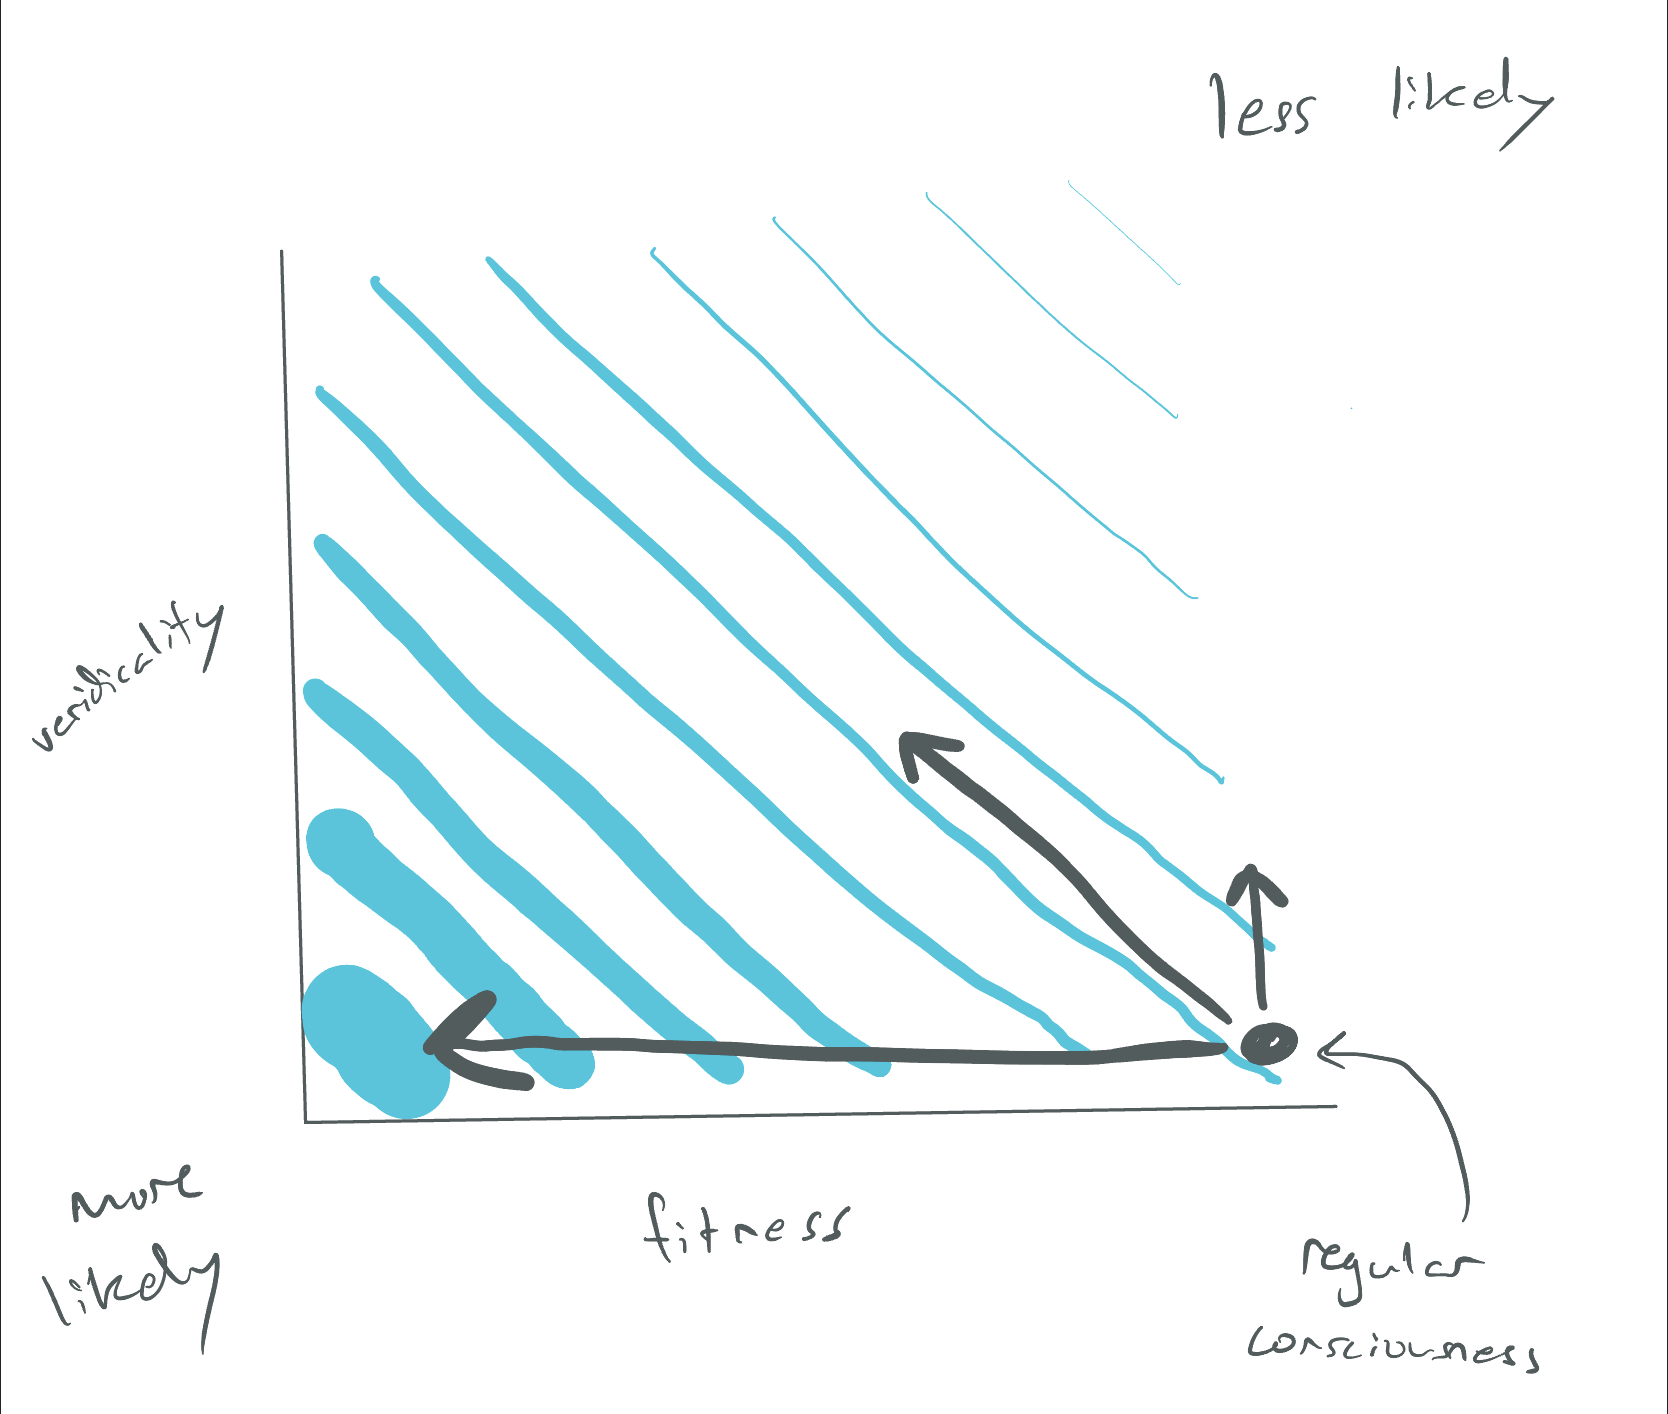
\includegraphics[scale = 0.2]{IMG_D69D74B327B2-1.jpeg}

\textcolor{red}{we can model a random change in consciousness as having a chance of either increasing or decreasing fitness and increasing or decreasing veridicality. See figure x. Random changes in concsciousness could mean a hit on the head, a change in hormones or perspective, or a drug.}

\textcolor{red}{\begin{itemize}
    \item rotating 3d mask optical illusion
    \item lowkey humans can echolocate
    \item the first phenomenon (mask) can be explained as a result of my experiment as it's just a more detailed version of sensory systems we already knew about, while the second is likely a still-functioning vestigial structure in which case my shit still kind of applies but also not really. It could be that the echolocation is slowly being phased out in which case my theory wouldn't apply. Or it could be that it has gone in and out of usefulness over the epochs in which case I am right.
\end{itemize}}

\textcolor{red}{I need to lay out the alternative interpretation of any related evidence (such as the two cases listed above) which says that maybe rather than that trait going in and out of usefulness it's just slowly going out of usefulness}


\bibliographystyle{apacite} 
\bibliography{bib.bib}

\end{document}
